%#! uplatex UserGuideJa
\chapter{後処理}
\label{chap:6}
\index{あとしょり@後処理}%
本章では,OpenFOAMでの後処理のオプションについて述べます.
OpenFOAMにはオープンソースの可視化アプリケーションである
\OFthirdparty{ParaView}を用いた後処理のユーティリティである
\OFtool{paraFoam}が提供されており,
これについては\autoref{sec:6.1}で述べています.
後処理の別の方法としては,
EnSightやFieldview等のサードパーティから供給されている製品を
使う方法やFluentの後処理を使う方法があります.



\section{\OFtool{paraFoam}}
\label{sec:6.1}
\index{paraFoam@\OFtool{paraFoam}}%
\index{あとしょり@後処理!paraFoam@\OFtool{paraFoam}}%
%%%
\OFrevision{要再訳}
\index{PVFoamReader@\OFclass{PVFoamReader}!ライブラリ}%
\index{ライブラリ!PVFoamReader@\OFclass{PVFoamReader}}%
\index{vtkFoam@\OFclass{vtkFoam}!ライブラリ}%
\index{ライブラリ!vtkFoam@\OFclass{vtkFoam}}%
%%%
OpenFOAMで提供されているメインの後処理用のツールは,
オープンソースの可視化アプリケーション\OFthirdparty{ParaView}から
OpenFOAMのデータを読み込めるようにするモジュールです.
このモジュールは,OpenFOAMにより提供されている\OFthirdparty{ParaView}の
バージョン4.1.0を用いている二つのライブラリである
\index{PV3FoamReader@\OFclass{PV3FoamReader}!ライブラリ}%
\index{ライブラリ!PV3FoamReader@\OFclass{PV3FoamReader}}%
\OFclass{PV3FoamReader}と
\index{vtkPV3Foam@\OFclass{vtkPV3Foam}!ライブラリ}%
\index{ライブラリ!vtkPV3Foam@\OFclass{vtkPV3Foam}}%
\OFclass{vtkPV3Foam}にコンパイルされています (バージョン
2.xの\OFthirdparty{ParaView}に対しては
\OFclass{PVFoamReader}および\OFclass{vtkFoam}です).
最新のバイナリでリリースされているソフトウエアについても適切に動作するはずですが,
このバージョンの\OFthirdparty{ParaView}をお使いになることを推奨します.
\OFthirdparty{ParaView}に関する詳細な内容およびドキュメントについては
\url{http://www.paraview.org}や
\url{http://www.kitware.com/products/paraviewguide.html}の
サイトから入手することができます.

\OFthirdparty{ParaView}はそのデータ処理とレンダリングのエンジンとして
Visualization Toolkit (\OFthirdparty{VTK}) を使っているため,
\OFthirdparty{VTK}フォーマットであれば,どのようなデータでも読み込むことができます.
OpenFOAMには\OFtool{foamToVTK}ユーティリティがあり,
ネイティブな書式のデータを\OFthirdparty{VTK}の書式に変換することができ,
つまりVTKベースの画像ツールであれば,OpenFOAMのケースの後処理として使うことができます.
これは,OpenFOAMで\OFthirdparty{ParaView}を使用する代替の手段となります.
ユーザには高度な使い方,並列処理における可視化を経験してほしいことから,
フリーのVisItを推奨します.
これは,\url{http://llnl.gov/visit/}から入手できます.

要約すると,OpenFoamの後処理用のツールとしては,
\OFthirdparty{ParaView}の読み込みモジュールを推奨します.
代わりの方法としては,OpenFOAMのデータを\OFthirdparty{ParaView}に読み込ませるために
\OFthirdparty{VTK}フォーマットに変換する方法と,
VTKベースのグラフィックツールを用いる方法があります.


\subsection{\OFtool{paraFoam}の概要}
\label{ssec:6.1.1}
\OFtool{paraFoam}は厳密には,
OpenFOAMで提供されている読み込みモジュールを用いて
\OFthirdparty{ParaView}を立ち上げるスクリプトです.
他のOpenFOAMのユーティリティ同様に,
ケースディレクトリ内からコマンド一つだけで,
あるいは引数として\texttt{-case}オプションでケース・パスを付けて,
実行します.
\begin{OFverbatim}[terminal]
paraFoam -case <caseDir>
\end{OFverbatim}
\OFthirdparty{ParaView}が立ち上がり,オープンすると\autoref{fig:6.1}のようになります.
ケースは左側のパネルでコントロールされますが,
それには次のような項目があります.
\begin{description}
 \item[\PVwindow{Pipeline Browser}]
\index{Pipeline Browser@\PVwindow{Pipeline Browser}!ウィンドウ}%
\index{ウィンドウ!Pipeline Browser@\PVwindow{Pipeline Browser}}%
            は,\OFthirdparty{ParaView}の中でオープンしているモジュールをリストアップしており,
            選択されたモジュールは青くハイライトされ,
            このモジュールに関するグラフィックスは,
            脇の目のボタンをクリックすることにより,
            有効・無効の切り替えができます.
 \item[\PVpanel{Properties}パネル]
\index{Properties@\PVpanel{Properties}!ウィンドウパネル}%
\index{ウィンドウパネル!Properties@\PVpanel{Properties}}%
            には,時間や領域,およびフィールドなどのケースに関する
            入力条件の選択項目があります.
 \item[\PVpanel{Display}パネル]
\index{Display@\PVpanel{Display}!ウィンドウパネル}%
\index{ウィンドウパネル!Display@\PVpanel{Display}}%
            は,色など,選択されたモジュールの可視化の表現をコントロールします.
 \item[\PVpanel{Information}パネル]
\index{Information@\PVpanel{Information}!ウィンドウパネル}%
\index{ウィンドウパネル!Information@\PVpanel{Information}}%
            はメッシュのジオメトリとサイズのようなケースの統計値を表示します.
\end{description}


\begin{figure}[ht]
 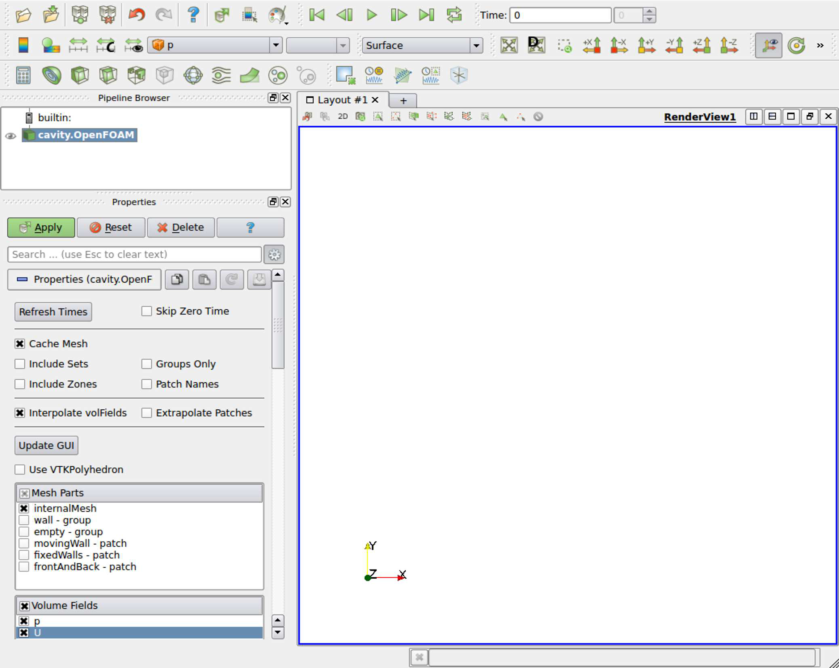
\includegraphics{fig-6-1}
 \caption{\OFtool{paraFoam}の画面}
 \label{fig:6.1}
\end{figure}


\OFthirdparty{ParaView}はツリー構成に基づいた構造で操作するようになっており,
その中で,トップレベルのケースのモジュールからサブモジュールのケースを
作成するフィルタをかけることができます.
例えば,圧力のコンタのプロットは,すべての圧力データをもつ
ケースモジュールのサブモジュールとすることができます.
\OFthirdparty{ParaView}の長所は,ユーザが数多くのサブモジュールを作ることができることと,
画像やアニメーションのどちらでも作ることができるという点にあります.
例えば,ソリッドのジオメトリ,メッシュおよび速度ベクトル,
圧力のコンタのプロットなどが追加できますし,
これらアイテムについては必要に応じてオン・オフすることができます.

基本的な操作方法は,まず必要な項目の選択を行い,
それから\PVpanel{Properties}パネルで緑色の
\index{Apply@\PVbutton{Apply}!ボタン}%
\index{ボタン!Apply@\PVbutton{Apply}}%
をクリックします.
そのほかのボタンとしては,
必要に応じてGUIをリセットできる
\index{Reset@\PVbutton{Reset}!ボタン}%
\index{ボタン!Reset@\PVbutton{Reset}}%
\PVbutton{Reset}ボタン,
アクティブになっているモジュールを削除する
\index{Delete@\PVbutton{Delete}!ボタン}%
\index{ボタン!Delete@\PVbutton{Delete}}%
\PVbutton{Delete}ボタンがあります.


\subsection{\PVpanel{Properties}パネル}
\label{ssec:6.1.2}
ケースモジュールの\PVpanel{Properties}パネルにはタイムステップや領域,
およびフィールドの設定の機能があります.
コントロール方法については,\autoref{fig:6.2}に説明を記載しています.
現在の読み込みモジュールにおいて,
ディレクトリ内のデータを\OFthirdparty{ParaView}に書き込むことは,特に価値はありません.
\autoref{ssec:6.1.4}節に書いてあるように,
現在の読み込みモジュールにおいて,
\index{Current Time Controls@\PVmenu{Current Time Controls}!メニュー}%
\index{メニュー!Current Time Controls@\PVmenu{Current Time Controls}}%
\PVmenu{Current Time Controls}あるいは
\index{VCR Controls@\PVmenu{VCR Controls}!メニュー}%
\index{メニュー!VCR Controls@\PVmenu{VCR Controls}}%
\PVmenu{VCR Controls}ツールバー内のボタンで,
表示のための時間データを選択することができます.
paraFoamの操作においては,
何らかの変更を行ったときには\PVbutton{Apply}をクリックする必要があります.
この\PVbutton{Apply}ボタンは,ユーザが変更するつもりがなかった場合を考慮して,
警告を与えるために緑色にハイライトされます.
この操作方法は,承諾する前に多くの選択ができるという長所をもっており,
特に,大きなケースでは,データ処理が最小限で行えるという便利さがあります.
しばしばファイルのケースデータが変更され,
(たとえばフィールドデータが新しい時間ディレクトリに書き込まれたりしたために)
\OFthirdparty{ParaView}を書き換える必要がある場合があります.
変更を書き込む際には,Propertiesパネル一番上の
\index{Update GUI@\PVbutton{Update GUI}!ボタン}%
\index{ボタン!Update GUI@\PVbutton{Update GUI}}%
\PVbutton{Update GUI}ボタンを
チェックすることによって変更します.


\begin{figure}[ht]
 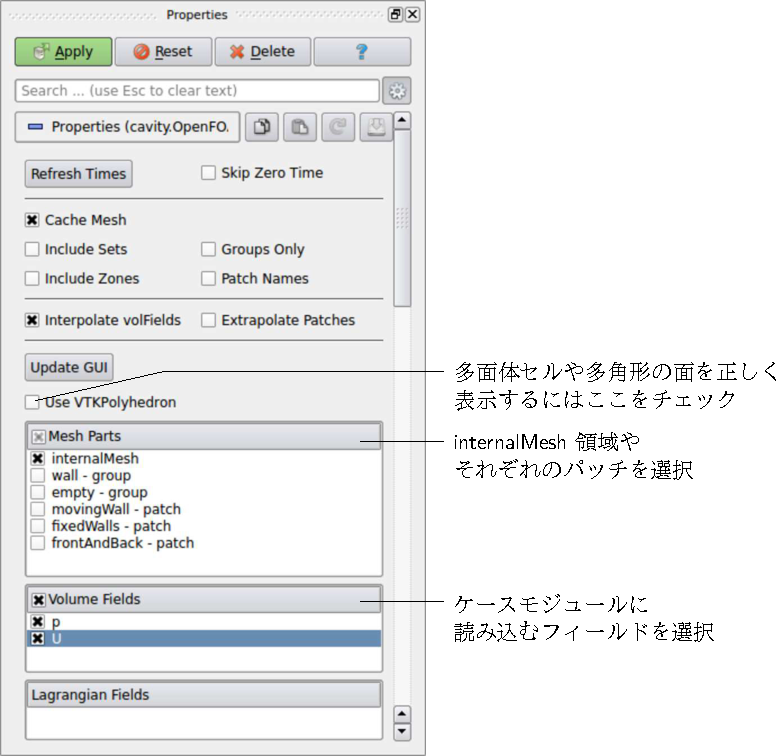
\includegraphics{fig-6-2}
 \caption{ケースモジュールのプロパティパネル}
 \label{fig:6.2}
\end{figure}


\subsection{\PVpanel{Display}パネル}
\label{ssec:6.1.3}
\index{Display@\PVpanel{Display}!ウィンドウパネル}%
\index{ウィンドウパネル!Display@\PVpanel{Display}}%
\PVpanel{Display}パネルには,与えられたケースモジュールのデータの
可視化に関する機能があります.


\begin{figure}[ht]
 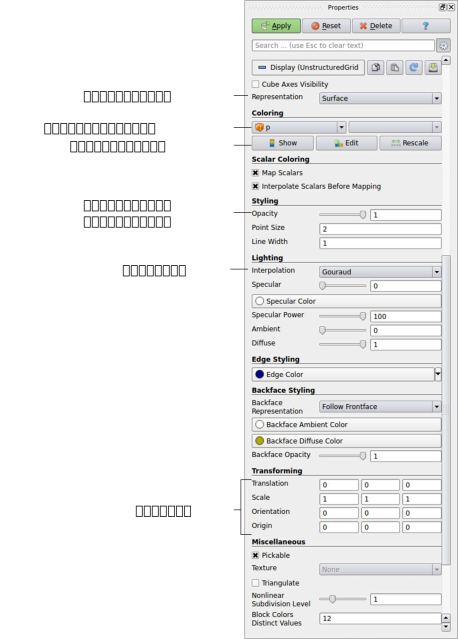
\includegraphics{fig-6-3}
 \caption{Displayパネル}
 \label{fig:6.3}
\end{figure}


以下が特に重要な点です.
\begin{itemize}
 \item データのレンジは,フィールドの最大値・最小値に対して
       自動的に更新はされませんので,
       特に,初期のケースモジュールをロードしたときには,
       適切なインターバルをRescale to Data Rangeで
       選択するように注意する必要があります.
 \item
\index{Edit Color Map@\PVbutton{Edit Color Map}!ボタン}%
\index{ボタン!Edit Color Map@\PVbutton{Edit Color Map}}%
      \PVbutton{Edit Color Map}ボタンでは,二つのパネルによるウィンドウが開きます.
       \begin{enumerate}
        \item
\index{Color Scale@\PVpanel{Color Scale}!ウィンドウパネル}%
\index{ウィンドウパネル!Color Scale@\PVpanel{Color Scale}}%
             \PVpanel{Color Scale}パネルではスケールの色を選択することができます.
              標準の青〜赤のCFDスケールを選択するには,
\index{Choose Preset@\PVbutton{Choose Preset}!ボタン}%
\index{ボタン!Choose Preset@\PVbutton{Choose Preset}}%
              \PVbutton{Choose Preset}をクリックし,Blue to Red Rainbox HSVを選択します.
        \item
\index{Color Legend@\PVpanel{Color Legend}!ウィンドウパネル}%
\index{ウィンドウパネル!Color Legend@\PVpanel{Color Legend}}%
             \PVpanel{Color Legend}パネルではカラーバーの凡例の色を切り替えたり,
              フォントのような凡例のレイアウトを決定します.
       \end{enumerate}
 \item 基本となるメッシュは
\index{Style@\PVpanel{Style}!ウィンドウパネル}%
\index{ウィンドウパネル!Style@\PVpanel{Style}}%
       \PVpanel{Style}パネルにある\PVmenu{Representation}メニューの
\index{Wrireframe@\PVmenu{Wrireframe}!メニューエントリ}%
\index{メニューエントリ!Wrireframe@\PVmenu{Wrireframe}}%
       \PVmenu{Wrireframe}を選択することにより表示されます.
 \item \PVmenu{Wrireframe}が選択されている場合のメッシュのようなジオメトリは
\index{Color By@\PVmenu{Color By}!メニュー}%
\index{メニュー!Color By@\PVmenu{Color By}}%
       \PVmenu{Color By}メニューから
\index{Solid Color@\PVmenu{Solid Color}!メニューエントリ}%
\index{メニューエントリ!Solid Color@\PVmenu{Solid Color}}%
       \PVmenu{Solid Color}を選択し,
\index{Set Ambient Color@\PVbutton{Set Ambient Color}!ボタン}%
\index{ボタン!Set Ambient Color@\PVbutton{Set Ambient Color}}%
       \PVbutton{Set Ambient Color}ウィンドウで色を指定することにより可視化することができます.
 \item イメージは
\index{Opacity@\PVpanel{Opacity}!テキストボックス}%
\index{テキストボックス!Opacity@\PVpanel{Opacity}}%
       \PVpanel{Opacity}の値 ($1 = \mbox{solid}$,$0 = \mbox{invisible}$) を
       修正することにより半透明にすることができます.
\end{itemize}


\subsection{ボタンツールバー}
\label{ssec:6.1.4}
\OFthirdparty{ParaView}の各機能はメインウインドウ上部の
メニューバーのプルダウンメニューだけでなく,
その下にあるボタンツールバーから選択することもできます.
表示するツールバーは
\index{View@\PVmenu{View}!メニュー}%
\index{メニュー!View@\PVmenu{View}}%
\PVmenu{View}メニューの
\index{Toolbars@\PVmenu{Toolbars}!メニューエントリ}%
\index{メニューエントリ!Toolbars@\PVmenu{Toolbars}}%
\PVmenu{Toolbars}から選択することができます.
各ツールバーの初期設定の配置は\autoref{fig:6.4}のようになっており,
それぞれどのプルダウンメニューの項目に対応するかを示しています.
多くのボタンの機能はアイコンから明快ですし,
\index{Help@\PVmenu{Help}!メニュー}%
\index{メニュー!Help@\PVmenu{Help}}%
\PVmenu{Help}メニューのtooltipsにチェックがされていれば
ポインタを上に置いたときに簡潔な注を表示させることができます.


\begin{figure}[ht]
 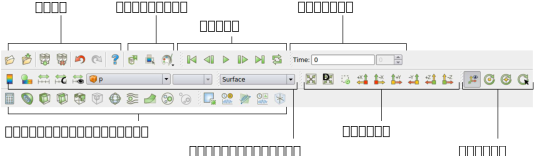
\includegraphics{fig-6-4}
 \caption{\OFthirdparty{ParaView}のツールバー}
 \label{fig:6.4}
\end{figure}


\subsection{表示の操作}
\label{ssec:6.1.5}
本節では,\OFtool{paraFoam}におけるオブジェクトの
表示の設定と取り扱いに関する操作について説明します.

\subsubsection{表示の設定}
\label{sssec:6.1.5.1}
\index{View Settings@\PVmenu{View Settings}!メニューエントリ}%
\index{メニューエントリ!View Settings@\PVmenu{View Settings}}%
\PVmenu{View Settings}を
\index{Edit@\PVmenu{Edit}!メニュー}%
\index{メニュー!Edit@\PVmenu{Edit}}%
\PVmenu{Edit}メニューから選択すると,
\index{General@\PVpanel{General}!ウィンドウパネル}%
\index{ウィンドウパネル!General@\PVpanel{General}}%
\PVpanel{General},
\index{Lights@\PVpanel{Lights}!ウィンドウパネル}%
\index{ウィンドウパネル!Lights@\PVpanel{Lights}}%
\PVpanel{Lights},
\index{Annotation@\PVpanel{Annotation}!ウィンドウパネル}%
\index{ウィンドウパネル!Annotation@\PVpanel{Annotation}}%
\PVpanel{Annotation}の3項目からなる
\index{View Settings (Render View)@\PVwindow{View Settings (Render View)}!ウィンドウ}%
\index{ウィンドウ!View Settings (Render View)@\PVwindow{View Settings (Render View)}}%
\PVwindow{View Settings (Render View)}ウインドウが表示されます.
\PVpanel{General}には以下のような項目がありますので,
開始時に設定するとよいでしょう.
\begin{itemize}
 \item 背景色としては,印刷物には白が望ましいでしょう.
       そのためには\PVbutton{Choose Color}ボタンの横の下向き矢印から
       \PVbutton{background}を選択した後で,
       \PVbutton{Choose Color}ボタンをクリックして色を選択します.
 \item CFD,特に2次元のケースでは
\index{Use Parallel Projection@\PVbutton{Use Parallel Projection}!ボタン}%
\index{ボタン!Use Parallel Projection@\PVbutton{Use Parallel Projection}}%
       \PVbutton{Use Parallel Projection}(平行投影)がよく用いられます.
\end{itemize}

\PVpanel{Lights}パネルに含まれる\PVpanel{Light Kit}パネルでは光源の詳細設定ができます.
\PVpanel{Headlight}パネルでは直接光をコントロールします.
\PVbutton{Headlight}ボタンを白色光の強度1にすれば,
等値面などの鮮明な色の画像を得られるでしょう.

\PVpanel{Annotation}では,表示ウィンドウにおける
軸や原点などの注釈の表示の有無を設定します.
\index{Orientation Axes@\PVbutton{Orientation Axes}!ボタン}%
\index{ボタン!Orientation Axes@\PVbutton{Orientation Axes}}%
\PVbutton{Orientation Axes}で$x$,$y$,$z$軸の色など,軸の表示設定をします.

\subsubsection{一般的な設定}
\label{sssec:6.1.5.2}
\index{Settings@\PVmenu{Settings}!メニューエントリ}%
\index{メニューエントリ!Settings@\PVmenu{Settings}}%
\PVmenu{Settings}を\PVmenu{Edit}メニューから選択すると
\index{General@\PVpanel{General}!ウィンドウパネル}%
\index{ウィンドウパネル!General@\PVpanel{General}}%
\PVpanel{General},
\index{Colors@\PVpanel{Colors}!ウィンドウパネル}%
\index{ウィンドウパネル!Colors@\PVpanel{Colors}}%
\PVpanel{Colors},
\index{Animations@\PVpanel{Animations}!ウィンドウパネル}%
\index{ウィンドウパネル!Animations@\PVpanel{Animations}!}%
\PVpanel{Animations},
\index{Charts@\PVpanel{Charts}!ウィンドウパネル}%
\index{ウィンドウパネル!Charts@\PVpanel{Charts}}%
\PVpanel{Charts},
および
\index{Render View@\PVpanel{Render View}!ウィンドウパネル}%
\index{ウィンドウパネル!Render View@\PVpanel{Render View}}%
\PVpanel{Render View}の項目からなる
\index{Options@\PVwindow{Options}!ウィンドウ}%
\index{ウィンドウ!Options@\PVwindow{Options}}%
\PVwindow{Options}ウインドウが表示されます.

\PVpanel{General}パネルでは\OFthirdparty{ParaView}の挙動の初期値を設定します.
特に,
\index{Auto Accept@\PVbutton{Auto Accept}!ボタン}%
\index{ボタン!Auto Accept@\PVbutton{Auto Accept}}%
\PVbutton{Auto Accept}をチェックすると
Propertiesウインドウで行った変更が
\index{Apply@\PVbutton{Apply}!ボタン}%
\index{ボタン!Apply@\PVbutton{Apply}}%
\PVbutton{Apply}ボタンをクリックすることなく
自動で表示に反映されるようになります.
大きな解析ケースではこのオプションは使わない方がよいでしょう.
というのもいくつもの変更を行う際にそのつど再描画されるのは煩わしく,
一度で反映させた方がよいと思われるからです.

\index{Render View@\PVpanel{Render View}!ウィンドウパネル}%
\index{ウィンドウパネル!Render View@\PVpanel{Render View}}%
\PVpanel{Render View}パネルには\PVpanel{General},
\PVpanel{Camera},\PVpanel{Server}の三つの項目があります.
\PVpanel{General}パネルではlevel of detail (LOD) で回転や平行移動,
サイズ変更といった操作時のレンダリングの精度を設定できます.
レベルを下げることで多数のセルからなるケースにおいても
視点操作時の再描画速度を早くすることができます.

\PVpanel{Camera}パネルでは3Dまたは2Dにおける視点の移動を設定します.
回転,平行移動,ズームといった操作は,マウスとshiftキー,
controlキーを組み合わせて行うことができますが,
割当ては任意に設定することができます.


\subsection{コンタのプロット}
\label{ssec:6.1.6}
コンタのプロットは,上部のメニューバーの\PVmenu{Filter}メニューから
\PVfilter{Contour}を選択することにより作成することができます.
フィルタはあたえられたモジュール上で役割を果たすことから,
モジュール自体が3Dのケースの場合には,コンタは一定の値を表す
2D表示(同値面:アイソサーフェス)に設定されます.
コンタに関する\PVpanel{Properties}にはユーザが編集できる\PVpanel{Isosurfaces}のリストがあり,
\PVwindow{New Range}ウィンドウにより使いやすくなっています.
スカラフィールドはプルダウンメニューにより選択することができます.

\subsubsection{断面の使い方}
\label{sssec:6.1.6.1}
同一面でのコンタの作成でなく,
断面のコンタを作成したい場合がよくあります.
そうするには,最初に\PVfilter{Slice}フィルタを用いて,
コンタをプロットしたい切断面を作成する必要があります.
この\PVfilter{Slice}フィルタでは,
ユーザは\PVkeyword{Slice Type}メニューで
\PVkeyword{Plane},\PVkeyword{Box}または\PVkeyword{Sphere}という
切断方法を指定することができます.
\OFrevision{古いキーワード?}%
それぞれ\PVentry{center}および\PVentry{normal}または\PVentry{radius}の指定が必要です.
マウスを使っても同じように切断面の操作を行うことができます.
そして\PVfilter{Contour}フィルタを実行すれば,
指定した切断面でコンタラインが作成されます.

\subsection{ベクトルのプロット}
\label{ssec:6.1.7}
ベクトルのプロットは\PVfilter{Glyph}フィルタを用いて作成します.
このフィルタは\PVentry{Vectors}で選択されたフィールドを読み込み,
いくつかの\PVentry{Glyph Types}が用意されていますが,
\PVentry{Arrow}によりクリアなベクトル画像が得られます.
それぞれのグリフには,
パネル上でユーザが操作して最も良い視覚効果を得るための,
描画をコントロールする選択肢が備わっています.

\PVpanel{Properties}パネルの残りの部分にある主要なものは
グリフの\PVentry{Scale Mode}メニューです.
その中でも最もよく使うオプションは,
グリフの長さがベクトルの大きさに比例する\PVentry{Vector},
全てのグリフを同じ長さにする\PVentry{Off}です.
また,\PVentry{Set Scale Factor}はグリフの基本的な長さをコントロールします.

\subsubsection{セルの中心でのプロット}
\label{sssec:6.1.7.1}
ベクトルは,デフォルトではセルの頂点上に作成されますが,
セルの中心にプロットデータを作成したい場合もあります.
このためには,まずそのケースモジュールに対して\PVfilter{Cell Centers}フィルタを適用し,
それから得られたセル中心データに対して\PVfilter{Glyph}フィルタを適用します.

\subsection{流線}
\label{ssec:6.1.8}
流線は,\PVfilter{Stream Tracer}フィルタを用いて作成された
トレーサラインを用いて作成されます.
トレーサの
\index{Seed@\PVpanel{Seed}!ウィンドウパネル}%
\index{ウィンドウパネル!Seed@\PVpanel{Seed}}%
\PVpanel{Seed}パネルで,\PVentry{Line Source}あるいは\PVentry{Point Cloud}全般の
トレーサポイントの配分を指定します.
ユーザは線のようなトレーサソースを見ることができますが,
白で表示させている場合は背景を変更しなければなりません.
トレーサの軌跡の間隔とトレーサのステップの長さは
\PVpanel{Stream Tracer}パネルの下にあるテキストボックスで指定します.
望み通りのトレーサのラインを作成するプロセスは大部分が試行錯誤であり,
ステップの長さを減少させることによりと同じように
円滑にはっきりと表示することができますが,反面計算時間が長くなります.
トレーサのラインが作成できた後は,
より高品質な画像を作り出すために\PVpanel{Tubes}フィルタを
\PVmodule{Tracer}モジュールに適用することができます.
このTubesは各々のトレーサのラインをたどっており,
厳密な円筒型にはなっていませんが,
固定された側面と半径の数値を持っています.
上述のように側面の数値が10に設定されたとき,
\PVfilter{Tubes}は円筒型として表示されますが,
やはり,これにも計算コストがかかります.


\subsection{画像の出力}
\label{ssec:6.1.9}
\OFthirdparty{ParaView}から画像を出力する最も簡単な方法は
\PVmenu{File}メニューから
\index{Save Screeshot@\PVmenu{Save Screeshot}!メニューエントリ}%
\index{メニューエントリ!Save Screeshot@\PVmenu{Save Screeshot}}%
\PVmenu{Save Screeshot}を選択することです.
選択すると,保存する画像の解像度を指定するウインドウが現れます.
自動的に解像度が設定されるよう,
アスペクト比を固定するボタンがあります.
ピクセル解像度を設定すると画像が保存されます.
より高画質で保存するには,
$x$方向の解像度を1000以上にするとよいでしょう.
PDF文書などに挿入する際に,A4あるいはUSレターサイズなどの
書面に合うようにスケーリングすれば,
シャープな仕上がりになります.


\subsection{アニメーション出力}
\label{ssec:6.1.10}
アニメーションを作成するには,
まず\PVmenu{File}メニューから
\index{Save Animation@\PVmenu{Save Animation}!メニューエントリ}%
\index{メニューエントリ!Save Animation@\PVmenu{Save Animation}}%
\PVmenu{Save Animation}を選択します.
解像度などいくつかの項目を設定するダイアログウインドウが
表示されるので,必要な解像度を指定します.
それ以外では,タイムステップごとのフレーム数が重要です.
これは直感的には1と設定するでしょうが,
アニメーションのフレーム数を多くするために
より大きな値にしてもかまいません.
この方法は,特に\texttt{mpeg}など,動画プレイヤの再生速度に制限がある場合に,
アニメーションの速度を遅くしたいときに有効です.

\PVbutton{Save Animation}ボタンを押すと,
ファイル名やファイル形式を設定する別のウインドウが現れます.
OKを押すと,``\verb|<ファイル名>_<画像番号>.<拡張子>|'' という名前で
一群の画像ファイルが保存されます.
例えば,ファイル名を ``\verb|animation|'' として
\texttt{jpg}形式で保存した場合の3番目の画像は,
``\verb|animation_0002.jpg|'' となります.
(\verb|<画像番号>| は0000から始まります)

一連の画像が保存されると,
適当なソフトを使って動画に変換することができます.
ImageMagickパッケージに含まれる変換ユーティリティは,
以下のようにコマンドラインから実行できます.
\begin{OFverbatim}[terminal]
convert animation*jpg movie.mpg
\end{OFverbatim}
mpg動画を作成する際に初期設定の \verb|-quality 90%|から
動画のクオリティを上げるといいでしょう.
これによって粒状ノイズを削減することができます.



\section{\OFthirdparty{Fluent}による後処理}
\label{sec:6.2}
\OFthirdparty{Fluent}を,OpenFOAMで実行したケースに,
ポストプロセッサとして適用することも可能です.
その目的のために,二つの変換器が提供されています.
\index{foamMeshToFluent@\OFtool{foamMeshToFluent}!ユーティリティ}%
\index{ユーティリティ!foamMeshToFluent@\OFtool{foamMeshToFluent}}%
\OFtool{foamMeshToFluent}は,
OpenFOAMのメッシュを\OFthirdparty{Fluent}フォーマットに変換し,
それを\texttt{.msh}ファイルとして書き出します.
そして,
\index{foamDataToFluent@\OFtool{foamDataToFluent}!ユーティリティ}%
\index{ユーティリティ!foamDataToFluent@\OFtool{foamDataToFluent}}%
\OFtool{foamDataToFluent}は,OpenFOAMの結果のデータを,
\OFthirdparty{Fluent}が読むことができる\texttt{.dat}ファイルに変換します.
\OFtool{foamMeshToFluent}は,普通の方法で実行することができます.
その結果のメッシュは,そのケースディレクトリの
\index{fluentInterface@\OFpath{fluentInterface}!ディレクトリ}%
\index{ディレクトリ!fluentInterface@\OFpath{fluentInterface}}%
\OFpath{fluentInterface}サブディレクトリに書き出されます.
すなわち,\OFpath{<caseName>/fluentInterface/<caseName>.msh}です.

\OFtool{foamDataToFluent}は,OpenFOAMのデータの結果を,
\OFthirdparty{Fluent}フォーマットに変換します.
変換は,二つのファイルで制御します.
まず\OFdictionary{controlDict}ディクショナリに指定した\OFkeyword{startTime}が,
変換される計算結果の時刻となります.
最新の結果を変換したいならば
\OFkeyword{startFrom}を\OFkeyword{latestTime}と設定すればよいでしょう.
二つめは翻訳方法を指定する\OFpath{foamDataToFluentDict}ディクショナリです.
これは\OFpath{constant}ディレクトリ内に配置します.
この\OFpath{foamDataToFluentDict}ディクショナリの例を以下に示します.
\begin{OFverbatim}[file, linenum]
/*--------------------------------*- C++ -*----------------------------------*\
| =========                 |                                                 |
| \\      /  F ield         | OpenFOAM: The Open Source CFD Toolbox           |
|  \\    /   O peration     | Version:  2.3.0                                 |
|   \\  /    A nd           | Web:      www.OpenFOAM.org                      |
|    \\/     M anipulation  |                                                 |
\*---------------------------------------------------------------------------*/
FoamFile
{
    version    2.0;
    format     ascii;
    class      dictionary;
    location   "system";
    object     foamDataToFluentDict;
}
// * * * * * * * * * * * * * * * * * * * * * * * * * * * * * * * * * * * * * //

p               1;

U               2;

T               3;

h               4;

k               5;

epsilon         6;

alpha1        150;


// ************************************************************************* //
\end{OFverbatim}
ディクショナリは,次の形式のエントリを含んでいます.
\begin{OFverbatim}[file]
<fieldName> <fluentUnitNumber>
\end{OFverbatim}
\verb|<fluentUnitNumber>|は,\OFthirdparty{Fluent}ポストプロセッサが使うラベルです.
\OFthirdparty{Fluent}は,ある決まったセットのフィールドしか認識しません.
\verb|<fluentUnitNumber>|の数の基本的なセットは,
\autoref{tbl:6.1}に引用されています.


\begin{table}[ht]
 %#! uplatex UserGuideJa
\begin{tabular}{lcc}
 Fluent名 & ユニット番号 & OpenFOAMでの一般名 \\
 \hline
 \tblstrut
 PRESSURE & 1 & \OFkeyword{p} \\
 MOMENTUM & 2 & \OFkeyword{U} \\
 TEMPERATURE & 3 & \OFkeyword{T} \\
 ENTHALPY & 4 & \OFkeyword{h} \\
 TKE & 5 & \OFkeyword{k} \\
 TED & 6 & \OFkeyword{epsilon} \\
 SPECIES & 7 & --- \\
 G & 8 & --- \\
 XF RF DATA VOF & 150 & \OFkeyword{gamma} \\
 TOTAL PRESSURE & 192 & --- \\
 TOTAL TEMPERATURE & 193 & --- \\
 \hline
\end{tabular}

 \caption{ポストプロセッサのための\OFthirdparty{Fluent}のユニット番号}
 \label{tbl:6.1}
\end{table}


ディクショナリは,ユーザがポストプロセスに必要とする,
全てのエントリを含まなければなりません.
たとえば,我々の例では,圧力\OFkeyword{p}と速度\OFkeyword{U}のためのエントリをいれています.
デフォルトエントリのリストは,\autoref{tbl:6.1}に記述されています.
ユーザは,他のユーティリティのように,
\OFtool{foamDataToFluent}を実行することができます.

\OFthirdparty{Fluent}でその結果を見るためには,
ケースのディレクトリの\OFpath{fluentInterface}サブディレクトリに移動して,
3次元のバージョンの\OFthirdparty{Fluent}を次のようにして開始します.
\begin{OFverbatim}[terminal]
fluent 3d
\end{OFverbatim}
メッシュとデータファイルは,ロードされ,その結果が可視化されます.
メッシュは,FileメニューのRead Caseを選択することで読むことができます.
あるデータタイプを読むためには,サポートアイテムを選択するべきです.
例えば,\OFkeyword{k}と\OFkeyword{epsilon}の乱流データを読むには,ユーザは,
\texttt{Define -> Models -> Viscous}メニューから
\texttt{k-epsilon}を選択することになります.
次に,データファイルは,\texttt{File}メニューの\texttt{Read Data}を選択することで,
読むことができます.

注意すべき点:ユーザは,OpenFOAM形式への変換に使われた
オリジナルの\OFthirdparty{Fluent}メッシュファイルを,
OpenFOAMの解を\OFthirdparty{Fluent}フォーマットに変換したものと
合わせて使ってはなりません.
なぜなら,ゾーンの番号付けの順序が保証できないからです.



\section{Fieldviewによる後処理}
\label{sec:6.3}
OpenFOAMは,OpenFOAMのケースを
Fieldviewでポストプロセスするための機能を提供しています.
後処理ユーティリティの\OFtool{foamToFieldview}を使って,
OpenFOAMのケースデータをFieldview \texttt{.uns}ファイルの形式に
変換することができます.

\OFtool{foamToFieldview}は,
他のOpenFOAMのユーティリティと同じように実行することができます.
\OFtool{foamToFieldview}は\OFpath{Fieldview}というディレクトリを
ケースディレクトリの中に作成します.
すでに\OFpath{Fieldview}ディレクトリが存在していた場合は削除されます.

デフォルトでは,\OFtool{foamToFieldview}は全ての
\OFpath{time}ディレクトリのデータを読み込んで,\break
\OFpath{<case>\_nn.uns}のようなファイルのセットに出力します.
\OFpath{nn}は連番で,最初の\OFpath{time}ディレクトリの
時刻歴データでは1から始まり,その後2,3,4と続きます.

ユーザーは,オプション \verb|-time <time>| を使用して,
特定の\OFpath{time}ディレクトリのデータだけを変換することもできます.
\verb|<time>| は,一般的,科学的,または固定の形式です.

Fieldviewの一部の機能は,境界条件に関する情報を必要とします.
たとえば流線を計算するとき,境界面についての情報を使用します.
\OFtool{foamToFieldview}はデフォルトで境界面の情報を含むように試みます.
ユーザは,コマンドオプション \verb|-noWall|を使って,
境界面情報を含まないように変換することもできます.

Fieldviewのunsファイルの拡張子は\texttt{.uns}です.
変換元となったOpenFOAMのケース名にドット \texttt{.} を含んでいる場合,
Fieldviewは一連のデータを時系列データと解釈することができず,
単一のデータ(定常データ)とみなすかもしれません.



\section{EnSightによる後処理}
\label{sec:6.4}
\OFtool{foamToEnsight}を使ってOpenFOAMのデータを
EnSightの形式に変換するか,\break
\OFtool{ensight74FoamExec}モジュールを使って
直接EnSightから読み込むことによって
EnSightで後処理を行うことができます.


\subsection{EnSightの形式への変換}
\label{ssec:6.4.1}
\OFtool{foamToEnSight}はOpenFOAMのデータをEnSightの形式に変換します.
\OFtool{foamToEnSight}は普通のアプリケーションと同様に実行できます.
\OFtool{foamToEnsight}はケースディレクトリ内に
\OFpath{Ensight}というディレクトリを作成します.
この際,既存の\OFpath{Ensight}ディレクトリは削除されます.
各時刻のディレクトリを読み込み,
ケースファイルとデータファイルのまとまりとして書き込みます.
ケースファイルは\OFpath{EnSight\_Case}という名前で
データファイルの詳細が含まれます.
各データファイルは\OFpath{EnSight\_nn.ext}という名前で,
\OFpath{nn}は最初の時間ディレクトリの時刻を\OFpath{1}として通し番号が入ります.
\OFpath{ext}は物理量に応じた拡張子です.
たとえば,\OFpath{T}は温度で,\OFpath{mesh}はメッシュです.
変換が完了するとEnSightで通常の方法で読み込むことができます.
\begin{itemize}
 \item EnSightのGUIにおいて,\texttt{File -> Data (Reader)} を選択する.
 \item ファイルボックス内で適切な\OFpath{EnSight\_Case}ファイルを強調表示させる.
 \item Formatの選択肢は,EnSightのデフォルトのCaseです.
 \item Caseをクリックし,Okayを選択する.
\end{itemize}


\subsection{\OFtool{ensight74FoamExec} readerモジュール}
\label{ssec:6.4.2}
\index{ensight74FoamExec@\OFtool{ensight74FoamExec}!ユーティリティ}%
\index{ユーティリティ!ensight74FoamExec@\OFtool{ensight74FoamExec}}%
EnSightではユーザ定義のモジュールを用いて他の形式のファイルを
EnSightに変換することが可能です.
OpneFOAMには\OFtool{ensight74FoamExec}というモジュールが
libuserd-foamライブラリにコンパイルされています.
EnSightに必要なのはこのライブラリで,
次節で述べるファイルシステムに置かれる必要があります.

\subsubsection{EnSightの読込モジュールの設定}
\label{sssec:6.4.2.1}
EnSightリーダの実行には,環境変数が適切である必要があります.
\OFpath{\$WM\_PROJECT\_\allowbreak DIR/\allowbreak etc/apps/\allowbreak ensightFoam}内の
\OFpath{bashrc}または\OFpath{cshrc}ファイルで設定を行います.
EnSightに関する環境変数は\autoref{tbl:6.2}の\verb|$CEI_|や\verb|$ENSIGHT7_|です.
EnSightの通常インストール時のパス設定では,
\verb|$CEI_HOME|のみ手動で設定すればよいはずです.%$


\begin{table}[ht]
 %#! uplatex UserGuideJa
\begin{tabularx}{\textwidth}{lX}
 環境変数 & 説明とオプション \\
 \hline
 \tblstrut
\index{CEI HOME@\string\OFenv{CEI\_HOME}!かんきょうへんすう@環境変数}%
\index{かんきょうへんすう@環境変数!CEI HOME@\string\OFenv{CEI\_HOME}}%
 \OFenv{\$CEI\_HOME} &
     EnSightがインストールされるパス(例:\OFpath{/usr/local/ensight})はデフォルトでシステムパスに加わる \\
\index{CEI ARCH@\string\OFenv{CEI\_ARCH}!かんきょうへんすう@環境変数}%
\index{かんきょうへんすう@環境変数!CEI ARCH@\string\OFenv{CEI\_ARCH}}%
 \OFenv{\$CEI\_ARCH} &
     \OFpath{\$CEI\_HOME/ensight74/machines}の
     マシンディレクトリ名に対応する名前から選択したマシン構造.
     デフォルト設定では\verb|linux_2.4|と\verb|sgi_6.5_n32|を含む \\
\index{ENSIGHT7 READER@\string\OFenv{ENSIGHT7\_READER}!かんきょうへんすう@環境変数}%
\index{かんきょうへんすう@環境変数!ENSIGHT7 READER@\string\OFenv{ENSIGHT7\_READER}}%
 \OFenv{\$ENSIGHT7\_READER} &
     EnSightがユーザの定義したlibuserd-foam読込みライブラリを探すパス,
     デフォルトでは\OFenv{\$FOAM\_LIBBIN}に設定 \\
\index{ENSIGHT7 INPUT@\string\OFenv{ENSIGHT7\_INPUT}!かんきょうへんすう@環境変数}%
\index{かんきょうへんすう@環境変数!ENSIGHT7 INPUT@\string\OFenv{ENSIGHT7\_INPUT}}%
 \OFenv{\$ENSIGHT7\_INPUT} &
     デフォルトでは\texttt{dummy}に設定 \\
 \hline
\end{tabularx}

 \caption{EnSightで用いる環境変数の設定}
 \label{tbl:6.2}
\end{table}


\subsubsection{読込モジュールの利用}
\label{sssec:6.4.2.2}
EnSight readerを使う際の主要な問題は,
解析ケースをOpenFOAMではディレクトリで定義するのに対し,
EnSightでは特定のファイルによって定義されている必要があるということです.
EnSightはディレクトリ名の選択ができないので,
以下の手順で,特にケースの詳細を選択する際に注意しながら
読込モジュールを使います.
\begin{enumerate}
 \item EnSightのGUIにおいて,\texttt{File -> Data (Reader)} を選択します.
 \item FormatメニューからOpenFOAMの選択ができるはずです.
       できない場合は,環境変数の設定に問題があります.
 \item File Selectionウインドウからケースディレクトリを探し,
       Directories欄の \verb|/.| または \verb|/..| で終わる,
       上二つのうち一つを強調表示させ,
       (Set) Geometryを選択します.
 \item パスフィールドには解析ケースが入っています.
       (Set) Geometryの欄には/が含まれるはずです.
 \item OkayをクリックするとEnSightがデータを読み込み始めます.
 \item データが読込まれると,新しくData Part Loaderウインドウが現れ,
       どの部分を読込むか尋ねられるので,Load allを選択します.
 \item Data Part Loaderのウインドウが表示されていると
       いくつかの機能が動かないので,
       メッシュがEnSightのウインドウに表示されたら閉じます.
\end{enumerate}



\section{データのサンプリング}
\label{sec:6.5}
OpenFOAMはフィールドデータの任意の位置における
値を取得するユーティリティ,
\index{sample@\OFtool{sample}!ユーティリティ}%
\index{ユーティリティ!sample@\OFtool{sample}}%
\OFtool{sample}を提供しています.
グラフ上にプロットするために1次元の線上,
または等値面画像を表示するために2次元平面上のデータが取得されます.
データ取得位置は,ケースの\OFpath{system}ディレクトリにある,
\OFpath{sampleDict}で指定します.
データは良く知られているグラフパッケージ,
Grace/xmgr,gnuplot,jPlotのような様々な形式で書き出すことができます.

\OFpath{sampleDict}ディクショナリは,
\OFpath{\$FOAM\_UTILITIES/postProcessing/sampling/sample}の
\OFpath{sample}ソースコードディレクトリにある
\/\OFpath{sampleDict}の例をコピーすることで作成できます.
\/\OFpath{\$FOAM\_\allowbreak TUTORIALS/\allowbreak solidDisplacementFoam}の
\OFpath{plateHole}チュートリアルのケースにも
1D線型データ取得のための記述例があります.
\begin{OFverbatim}[file, linenum=17]

interpolationScheme cellPoint;

setFormat       raw;

sets
(
    leftPatch
    {
        type    uniform;
        axis    y;
        start   ( 0 0.5 0.25 );
        end     ( 0 2 0.25 );
        nPoints 100;
    }
);

fields          ( sigmaxx );


// ************************************************************************* //
\end{OFverbatim}


\begin{table}[ht]
 %#! uplatex UserGuideJa
\begin{tabularx}{\textwidth}{llX}
 キーワード & オプション & 説明 \\
 \hline
 \tblstrut
\index{interpolationScheme@\string\OFkeyword{interpolationScheme}!キーワード}%
\index{キーワード!interpolationScheme@\string\OFkeyword{interpolationScheme}}%
 \OFkeyword{interpolationScheme} &
\index{cell@\string\OFkeyword{cell}!キーワードエントリ}%
\index{キーワードエントリ!cell@\string\OFkeyword{cell}}%
     \OFkeyword{cell} &
         セル中心の値でセル全体が一定とみなす \\
 &
\index{cellPoint@\string\OFkeyword{cellPoint}!キーワードエントリ}%
\index{キーワードエントリ!cellPoint@\string\OFkeyword{cellPoint}}%
     \OFkeyword{cellPoint} &
         セルの値から線型重み付け補間 \\
 &
\index{cellPointFace@\string\OFkeyword{cellPointFace}!キーワードエントリ}%
\index{キーワードエントリ!cellPointFace@\string\OFkeyword{cellPointFace}}%
     \OFkeyword{cellPointFace} &
         線型重み付けまたはセル界面から補間 \\
\index{setFormat@\string\OFkeyword{setFormat}!キーワード}%
\index{キーワード!setFormat@\string\OFkeyword{setFormat}}%
 \OFkeyword{setFormat} &
\index{raw@\string\OFkeyword{raw}!キーワードエントリ}%
\index{キーワードエントリ!raw@\string\OFkeyword{raw}}%
     \OFkeyword{raw} &
         ASCII生データ \\
 &
\index{gnuplot@\string\OFkeyword{gnuplot}!キーワードエントリ}%
\index{キーワードエントリ!gnuplot@\string\OFkeyword{gnuplot}}%
     \OFkeyword{gnuplot} &
         gnuplot形式データ \\
 &
\index{xmgr@\string\OFkeyword{xmgr}!キーワードエントリ}%
\index{キーワードエントリ!xmgr@\string\OFkeyword{xmgr}}%
     \OFkeyword{xmgr} &
         Grace/xmgr形式データ \\
 &
\index{jplot@\string\OFkeyword{jplot}!キーワードエントリ}%
\index{キーワードエントリ!jplot@\string\OFkeyword{jplot}}%
     \OFkeyword{jplot} &
         jPlot形式データ \\
\index{surfaceFormat@\string\OFkeyword{surfaceFormat}!キーワード}%
\index{キーワード!surfaceFormat@\string\OFkeyword{surfaceFormat}}%
 \OFkeyword{surfaceFormat} &
\index{null@\string\OFkeyword{null}!キーワードエントリ}%
\index{キーワードエントリ!null@\string\OFkeyword{null}}%
     \OFkeyword{null} &
         出力しない \\
 &
\index{foamFile@\string\OFkeyword{foamFile}!キーワードエントリ}%
\index{キーワードエントリ!foamFile@\string\OFkeyword{foamFile}}%
     \OFkeyword{foamFile} &
         点,面,値のファイル \\
 &
\index{dx@\string\OFkeyword{dx}!キーワードエントリ}%
\index{キーワードエントリ!dx@\string\OFkeyword{dx}}%
     \OFkeyword{dx} &
         DXスカラまたはベクトル形式 \\
 &
\index{vtk@\string\OFkeyword{vtk}!キーワードエントリ}%
\index{キーワードエントリ!vtk@\string\OFkeyword{vtk}}%
     \OFkeyword{vtk} &
         VTK ASCII形式 \\
 &
\index{raw@\string\OFkeyword{raw}!キーワードエントリ}%
\index{キーワードエントリ!raw@\string\OFkeyword{raw}}%
     \OFkeyword{raw} &
         $xyz$座標と値.gnuplotの\texttt{splot}などで使われる \\
 &
\index{stl@\string\OFkeyword{stl}!キーワードエントリ}%
\index{キーワードエントリ!stl@\string\OFkeyword{stl}}%
     \OFkeyword{stl} &
         ASCII STL.表面のみ,値なし \\
 \\
\index{fields@\string\OFkeyword{fields}!キーワード}%
\index{キーワード!fields@\string\OFkeyword{fields}}%
 \OFkeyword{fields} &
     \multicolumn{2}{l}{サンプルするフィールドのリスト,
     たとえば速度\OFkeyword{U}の場合,} \\
 &
     \OFkeyword{U} &
         $\bm{U}$の全成分を出力 \\
 \\
\index{sets@\string\OFkeyword{sets}!キーワード}%
\index{キーワード!sets@\string\OFkeyword{sets}}%
 \OFkeyword{sets} &
     \multicolumn{2}{l}{1次元のsetsサブディクショナリのリスト.\autoref{tbl:6.4}を参照} \\
\index{surfaces@\string\OFkeyword{surfaces}!キーワード}%
\index{キーワード!surfaces@\string\OFkeyword{surfaces}}%
 \OFkeyword{surfaces} &
     \multicolumn{2}{l}{2次元のsurfacesサブディクショナリリスト.
     \autoref{tbl:6.5}および\autoref{tbl:6.6}を参照} \\
 \hline
\end{tabularx}

 \caption{\OFpath{sampleDict}におけるキーワード指定}
 \label{tbl:6.3}
\end{table}


このファイルには,次の入力項目があります.
\begin{description}
 \item[interpolationScheme] データ内挿のスキーム
 \item[sets] フィールドが線型サンプルされる (1D) 解析領域の中の位置
 \item[surfaces] フィールドが面型サンプルされる (2D) 解析領域の中の位置
 \item[setFormat] 線データ出力のフォーマット
 \item[surfaceFormat] 面データ出力のフォーマット
 \item[fields] サンプルされるフィールド
\end{description}

\OFkeyword{interpolationScheme}には,多面体の各セルを四面体に分割し,
サンプルされる値が四面体頂点の値から補間される
\OFkeyword{cellPoint}と\OFkeyword{cellPointFace}オプションがあります.
\OFkeyword{cellPoint}では,四面体の頂点は,多面体のセルの中心と,
面の頂点三つからなります.セルの中心と一致する頂点は,
セル中心のフィールド値を継承し,
他の頂点はセルの中心の値から内挿した値をとります.
\OFkeyword{cellPointFace}では,四面体頂点の内の一つが,
面の中心とも一致します.
面が交差するセルの中心での値による内挿スキームによって,
フィールド値を継承します.

ラインサンプリングのための\OFkeyword{setFormat}エントリは,
生データフォーマットと,グラフ描画パッケージのためのgnuplot,
Grace/xmgr,jPlotフォーマットがあります.
データは,ケースディレクトリの\OFpath{sets}ディレクトリに書き出されます.
そのディレクトリは,一連の時刻ディレクトリに分割され,
データファイルは,その中に格納されます.
各々のデータファイルは,フィールド名,サンプルセット名,
そして出力フォーマットに関係した拡張子をもつ名前が付けられます.
拡張子は,生データでは\texttt{.xy},Grace/xmgr用には\texttt{.agr},
jPlotには\texttt{.dat}となります.
gnuplotのフォーマットは,生の形式のデータと,
それに加えてコマンドファイルを含んでいます.
このコマンドファイルは,\texttt{.gplt}という拡張子をもち,
グラフを生成するためのものです.
\OFtool{sample}が実行されるときは,
既存の\OFpath{sets}ディレクトリが削除されるので注意してください.

サーフェスサンプリングのための\OFkeyword{surfaceFormat}エントリは,
生データフォーマットとグラフ描画パッケージのためのgnuplot,
Grace/xmgr,jPlotフォーマットがあります.
データは,ケースディレクトリの,
\OFpath{surfaces}ディレクトリに書き出されます.
そのディレクトリは時間ディレクトリに分割され,
データファイルは\OFpath{sets}と同様にその中に格納されます.

\OFkeyword{fields}リストは,
データを取得したいフィールドが記述されます.
\OFtool{sample}ユーティリティは,次の限定された関数を,
ベクトルやテンソルフィールドを修正することができるように,
解析することができます.例えば,\OFkeyword{U}のためには,
\begin{description}
 \item[\texttt{U.component($n$)}] これは,
            ベクトル(テンソル)の$n$番目の要素を書く.
            $n = 0, 1, \ldots$
 \item[\texttt{mag(U)}] これは,
            ベクトル(テンソル)の大きさを書く
\end{description}
\OFkeyword{sets}リストは,サンプルされるべきデータの位置の,
サブディクショナリで構成されます.
各サブディクショナリは,そのセットの名前に従って名前が付けられ,
\autoref{tbl:6.4}にも示すようにデータ取得位置に関する記述がなされます.

例えば,\OFkeyword{uniform}サンプリングは,
\OFkeyword{start}と\OFkeyword{end}ポイントで指定した直線上に,
均等に分割した$n$点でデータを取得します.
全ての\OFkeyword{sets}には,
\OFkeyword{type}とグラフ用の縦軸の長さを指定する
\OFkeyword{axis}キーワードを与えます.


\begin{table}[ht]
 %#! uplatex UserGuideJa
\begin{tabular}{ll*{6}c}
 & & \multicolumn{6}{c}{必要項目} \\
 サンプル型 & データ取得位置 &
         \rotatebox{90}{\OFkeyword{name}} &
         \rotatebox{90}{\OFkeyword{axis}} &
         \rotatebox{90}{\OFkeyword{start}} &
         \rotatebox{90}{\OFkeyword{end}} &
         \rotatebox{90}{\OFkeyword{nPoints}} &
         \rotatebox{90}{\OFkeyword{points}} \\
 \hline
 \tblstrut
\index{uniform@\OFkeyword{uniform}!キーワード}%
\index{キーワード!uniform@\OFkeyword{uniform}}%
 \OFkeyword{uniform} & 線上に一様配分 &
         \textbullet & \textbullet & \textbullet & \textbullet & \textbullet \\
\index{face@\OFkeyword{face}!キーワード}%
\index{キーワード!face@\OFkeyword{face}}%
 \OFkeyword{face} & 指定された線とセル界面の交点 &
         \textbullet & \textbullet & \textbullet & \textbullet \\
\index{midPoint@\OFkeyword{midPoint}!キーワード}%
\index{キーワード!midPoint@\OFkeyword{midPoint}}%
 \OFkeyword{midPoint} & 線と界面の交点と交点の中点 &
         \textbullet & \textbullet & \textbullet & \textbullet \\
\index{midPointAndFace@\OFkeyword{midPointAndFace}!キーワード}%
\index{キーワード!midPointAndFace@\OFkeyword{midPointAndFace}}%
 \OFkeyword{midPointAndFace} & 中点および界面 &
         \textbullet & \textbullet & \textbullet & \textbullet \\
\index{curve@\OFkeyword{curve}!キーワード}%
\index{キーワード!curve@\OFkeyword{curve}}%
 \OFkeyword{curve} & 曲線に沿った指定された点 &
         \textbullet & \textbullet & & & & \textbullet \\
\index{cloud@\OFkeyword{cloud}!キーワード}%
\index{キーワード!cloud@\OFkeyword{cloud}}%
 \OFkeyword{cloud} & 指定された点 &
         \textbullet & \textbullet & & & & \textbullet \\
 \hline
\end{tabular}

\begin{tabular}{llll} \\
 入力項目 & 説明 & \multicolumn{2}{l}{オプション} \\
 \hline
 \tblstrut
 \OFkeyword{type} & データ取得の型 & \multicolumn{2}{l}{上の一覧参照} \\
 \OFkeyword{axis} & Output of sample location &
\index{x@\OFkeyword{x}!キーワードエントリ}%
\index{キーワードエントリ!x@\OFkeyword{x}}%
         \OFkeyword{x} & $x$軸 \\
 & &
\index{y@\OFkeyword{y}!キーワードエントリ}%
\index{キーワードエントリ!y@\OFkeyword{y}}%
         \OFkeyword{y} & $y$軸 \\
 & &
\index{z@\OFkeyword{z}!キーワードエントリ}%
\index{キーワードエントリ!z@\OFkeyword{z}}%
         \OFkeyword{z} & $z$軸 \\
 & &
\index{xyz@\OFkeyword{xyz}!キーワードエントリ}%
\index{キーワードエントリ!xyz@\OFkeyword{xyz}}%
         \OFkeyword{xyz} & $xyz$軸 \\
 & &
\index{distance@\OFkeyword{distance}!キーワードエントリ}%
\index{キーワードエントリ!distance@\OFkeyword{distance}}%
         \OFkeyword{distance} & 点0からの距離 \\
 \OFkeyword{start} & データ取得線の始点 & \multicolumn{2}{l}{e.g. \OFkeyword{(0.0 0.0 0.0)}} \\
 \OFkeyword{end} & データ取得線の終点 & \multicolumn{2}{l}{e.g. \OFkeyword{(0.0 2.0 0.0)}} \\
 \OFkeyword{nPoints} & データ取得点の数 & \multicolumn{2}{l}{e.g. \OFkeyword{200}} \\
 \OFkeyword{points} & データ取得点一覧 \\
 \hline
\end{tabular}

 \caption{\OFsubdictionary{sets}サブディクショナリにおけるエントリ}
 \label{tbl:6.4}
\end{table}


\begin{table}[ht]
 %#! uplatex UserGuideJa
\begin{tabular}{lll}
 キーワード & 説明 & オプション \\
 \hline
 \tblstrut
 \OFkeyword{basePoint} & 平面上の点 & e.g. \OFkeyword{(0 0 0)} \\
 \OFkeyword{normalVector} & 平面の法線ベクトル & e.g. \OFkeyword{(1 0 0)} \\
 \OFkeyword{interpolate} & 補間の有無 & \OFkeyword{true}/\OFkeyword{false} \\
 \OFkeyword{triangulate} & 三角形で分割するか(オプション) & \OFkeyword{true}/\OFkeyword{false} \\
 \hline
\end{tabular}

 \caption{\OFsubdictionary{surfaces}サブディクショナリにおける
 \OFkeyword{surfaces用}のエントリ}
 \label{tbl:6.5}
\end{table}


\begin{table}[ht]
 %#! uplatex UserGuideJa
\begin{tabular}{lll}
 キーワード & 説明 & オプション \\
 \hline
 \tblstrut
 \OFkeyword{patchName} & パッチ名 & e.g. \OFkeyword{movingWall} \\
 \OFkeyword{interpolate} & データ補間の有無 & \OFkeyword{true}/\OFkeyword{false} \\
 \OFkeyword{triangulate} & 三角形で分割するか(オプション) & \OFkeyword{true}/\OFkeyword{false} \\
 \hline
\end{tabular}

 \caption{\OFsubdictionary{surfaces}サブディクショナリにおける
\index{patch@\string\OFkeyword{patch}!キーワードエントリ}%
\index{キーワードエントリ!patch@\string\OFkeyword{patch}}%
 \OFkeyword{patch}用のエントリ}
 \label{tbl:6.6}
\end{table}


\OFkeyword{surfaces}リストは,
データ取得位置のサブディクショナリのリストによって構成されます.
各サブディクショナリは,表面の名前に従った名前が付けられ,
\OFkeyword{type}で始まる一連の記述で構成されます.
平面上の点と法線ベクトルで定義され,
\autoref{tbl:6.5}に示される項目の記述がなされる
\OFkeyword{plane}か,
または,既存の境界パッチと一致し,
\autoref{tbl:6.6}に示される項目の記述がなされる
\OFkeyword{patch}のいずれかです.



\section{ジョブのモニタと管理}
\label{sec:6.6}
本節では,まず正しく実行されたOpenFOAMのジョブについて言及し,
\autoref{sec:3.3}節で説明したソルバの基本的な実行についてまで述べます.
\OFpath{\$WM\_PROJECT\_DIR/etc/controlDict}ファイルの
\OFsubdictionary{DebugSwitches}の,
\OFkeyword{level}デバッグスイッチが\OFkeyword{1}または\OFkeyword{2}(デフォルト)であったなら,
ソルバの実行時に方程式の解の状態を標準出力,
例えばスクリーンに出力します.
以下では\OFpath{cavity}チュートリアルを解く際の出力の
冒頭部分を例として挙げています.
ここから解かれる各々の方程式について,レポート行に,ソルバ名,
解かれる変数,その初期と最終の残差,
そして反復回数が書かれていることが読み取れます.
\begin{OFverbatim}[baselinestretch=1, leftskip=1em, weight=\scriptsize]
    Starting time loop

Time = 0.005

Max Courant Number = 0
BICCG: Solving for Ux, Initial residual = 1, Final residual = 2.96338e-06, No Iterations 8
ICCG: Solving for p, Initial residual = 1, Final residual = 4.9336e-07, No Iterations 35
time step continuity errors : sum local = 3.29376e-09, global = -6.41065e-20, cumulative = -6.41065e-20
ICCG: Solving for p, Initial residual = 0.47484, Final residual = 5.41068e-07, No Iterations 34
time step continuity errors : sum local = 6.60947e-09, global = -6.22619e-19, cumulative = -6.86725e-19
ExecutionTime = 0.14 s

Time = 0.01

Max Courant Number = 0.585722
BICCG: Solving for Ux, Initial residual = 0.148584, Final residual = 7.15711e-06, No Iterations 6
BICCG: Solving for Uy, Initial residual = 0.256618, Final residual = 8.94127e-06, No Iterations 6
ICCG: Solving for p, Initial residual = 0.37146, Final residual = 6.67464e-07, No Iterations 33
time step continuity errors : sum local = 6.34431e-09, global = 1.20603e-19, cumulative = -5.66122e-19
ICCG: Solving for p, Initial residual = 0.271556, Final residual = 3.69316e-07, No Iterations 33
time step continuity errors : sum local = 3.96176e-09, global = 6.9814e-20, cumulative = -4.96308e-19
ExecutionTime = 0.16 s

Time = 0.015

Max Courant Number = 0.758267
BICCG: Solving for Ux, Initial residual = 0.0448679, Final residual = 2.42301e-06, No Iterations 6
BICCG: Solving for Uy, Initial residual = 0.0782042, Final residual = 1.47009e-06, No Iterations 7
ICCG: Solving for p, Initial residual = 0.107474, Final residual = 4.8362e-07, No Iterations 32
time step continuity errors : sum local = 3.99028e-09, global = -5.69762e-19, cumulative = -1.06607e-18
ICCG: Solving for p, Initial residual = 0.0806771, Final residual = 9.47171e-07, No Iterations 31
time step continuity errors : sum local = 7.92176e-09, global = 1.07533e-19, cumulative = -9.58537e-19
ExecutionTime = 0.19 s
\end{OFverbatim}


\subsection{計算実行用の\OFtool{foamJob}スクリプト}
\label{ssec:6.6.1}
\index{foamJob@\OFtool{foamJob}!スクリプト/エイリアス}%
\index{スクリプト/エイリアス!foamJob@\OFtool{foamJob}}%
ユーザは,残差や反復回数,Courant数などが,レポートデータとして
スクリーンを流れるのを確認すれば十分かもしれません.
その代わりに,レポートをログファイルにリダイレクトすることで
計算速度を向上させることもできます.
このために\OFtool{foamJob}スクリプトは,
便利なオプションを提供しています.
\verb|<solver>|を指定して実行することで,
計算がバックグラウンドで実行され,
出力を\OFpath{log}という名前のファイルに記録します.
\begin{OFverbatim}[terminal]
foamJob <solver>
\end{OFverbatim}
その他のオプションは,\verb|foamJob -help|を実行することで見ることができます.
\OFpath{log}ファイルは,\OFthirdparty{UNIX} \OFthirdparty{tail}コマンドを用いることで
見たいときに見ることができます.
一般的には,followを意味する\verb|-f|オプションを
一緒に用いることで\OFpath{log}ファイルに新しいデータが
記録されるのを捉えることができます.
\begin{OFverbatim}[terminal]
tail -f log
\end{OFverbatim}


\subsection{計算モニタ用の\OFtool{foamLog}スクリプト}
\label{ssec:6.6.2}
\index{foamLog@\OFtool{foamLog}!スクリプト/エイリアス}%
\index{スクリプト/エイリアス!foamLog@\OFtool{foamLog}}%
\OFpath{log}ファイルを読むことで,
ジョブをモニタするには,限界があります.
特に,長い期間にわたって,傾向を抽出するのは困難です.
したがって,\OFtool{foamLog}スクリプトによって残差や反復回数,
Courant数のデータを抽出し,グラフにプロットできるように
一連のファイルとして出力することができます.
スクリプトは次のように実行します.
\begin{OFverbatim}[terminal]
foamLog <logFile>
\end{OFverbatim}
ファイルは,ケースディレクトリの\OFpath{logs}という名前の
サブディレクトリの中に保存されます.
各々のファイルは,\OFpath{<var>\_<subIter>}という名前が付けられます.
ここで,\texttt{<var>} は,ログファイルの中で指定される変数の名前で,
\texttt{<subIter>} は,そのタイムステップにおける繰り返し回数です.
解かれた変数に対して,初期残差はその変数名\texttt{<var>}をとり,
最終残差は\OFpath{<var>FinalRes}という名前をとります.
デフォルトでは,ファイルは,時刻と抽出された値という2列のフォーマットで表されます.

例として,\OFpath{cavity}チュートリアルでは,
解が定常状態に収束するのかを見るために,
観察したいのは$U_{x}$方程式の初期残差です.
この場合,\OFpath{logs/Ux\_0}ファイルからデータを取り出し,
\autoref{fig:6.5}のようにプロットします.
ここでは,残差は単調に収束許容値まで減少しているのが読み取れます.

\OFtool{foamLog}は,\OFpath{log}ファイルから,
うまくそれができるようにファイルを作成します.
\OFpath{cavity}チュートリアルの例では次のファイルがあります.
\begin{itemize}
 \item Courant数,\OFpath{Courant\_0}
 \item $U_{x}$方程式の初期と最終の残差である,
       \OFpath{Ux\_0}と\OFpath{UxFinalRes\_0},そして反復回数の
       \OFpath{UxIters\_0} (そしてこれと同等の$U_{y}$データ)
 \item 累積,全体そしてローカルの連続誤差.
       これは,$p$方程式ごとに出す.
       \OFpath{contCumulative\_0},\OFpath{contGlobal\_0},\OFpath{contLocal\_0},
       \OFpath{contCumulative\_1},\OFpath{contGlobal\_1},\OFpath{contLocal\_1}
 \item $p$方程式から,残差と反復回数\OFpath{p\_0}, \OFpath{pFinalRes\_0},
       \OFpath{pIters\_0},\OFpath{p\_1},\OFpath{pFinalRes\_1},\OFpath{pIters\_1}
 \item 実行時間,\OFpath{executionTime}
\end{itemize}


\begin{figure}[ht]
 \includegraphics{fig-6-5}
 \caption{\OFpath{cavity}チュートリアルにおける$U_{x}$の初期残差}
 \label{fig:6.5}
\end{figure}
